\section{Lösungskonzept} \label{sec:loesungskonzept}
\subsection{Problemstellung} \label{subsec:problemstellung}
Um eine erste Übersicht der möglichen Probleme des Lösungskonzepts zu erhalten, wurden folgende Punkte im Brainstormingverfahren zusammengetragen:
\begin{figure}[h]
	\centering
	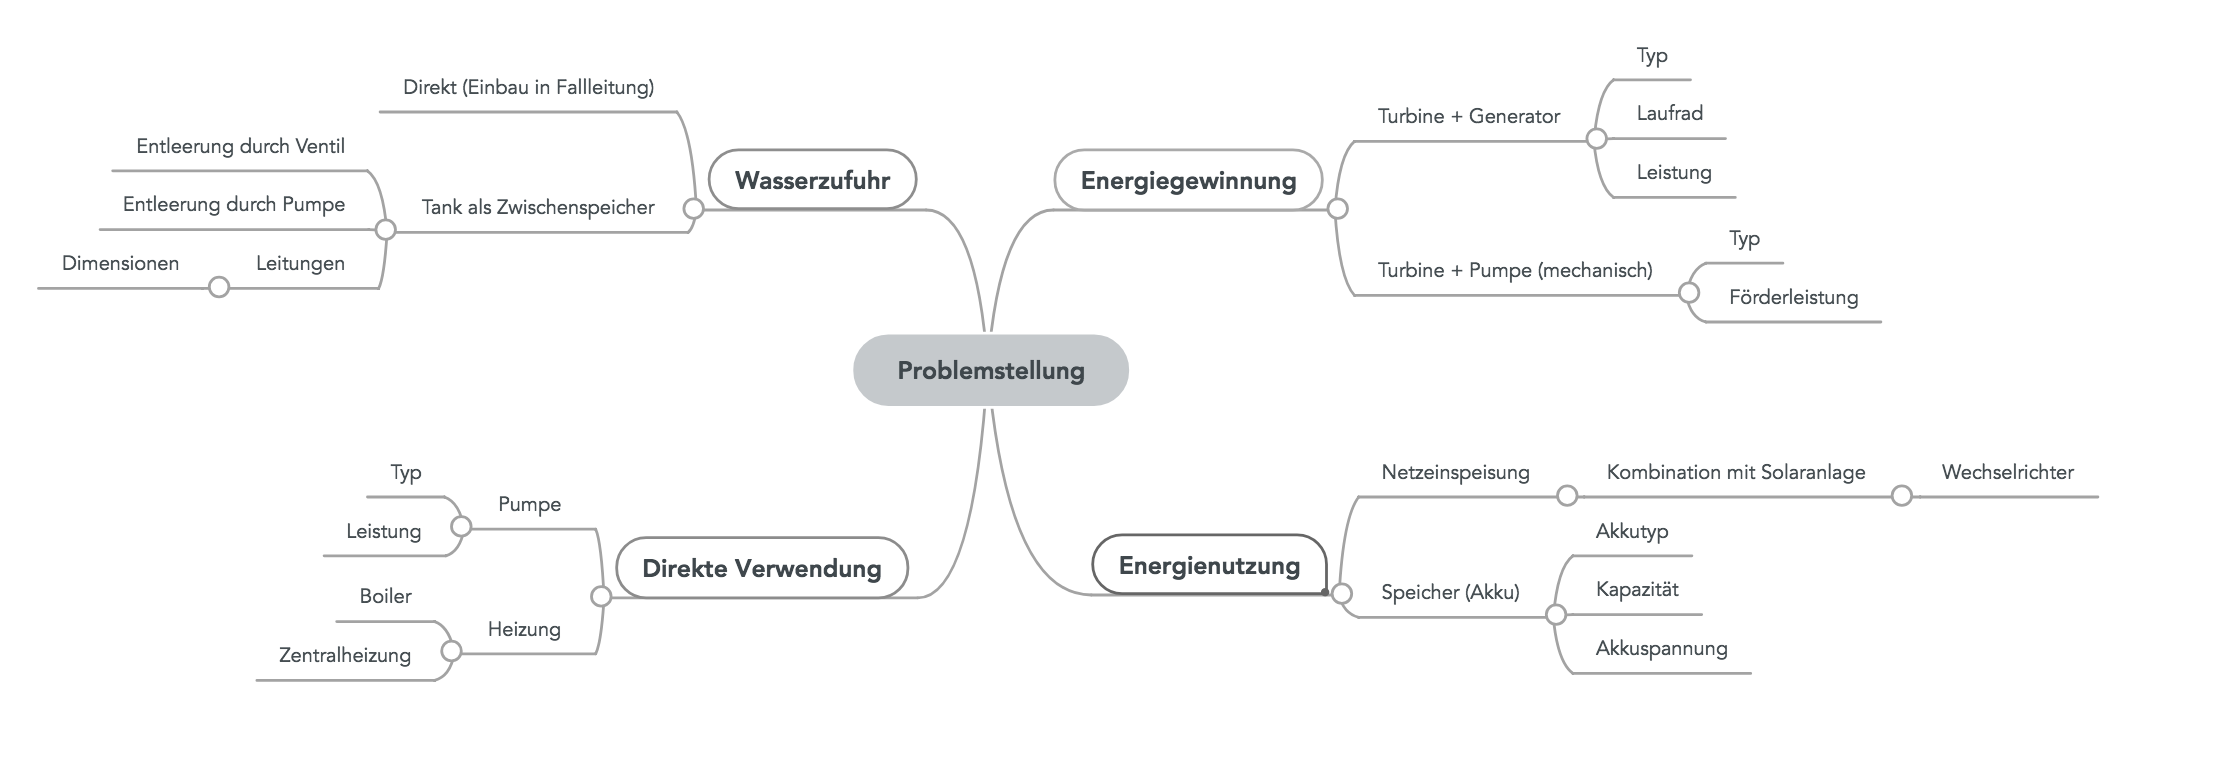
\includegraphics[width=0.9\linewidth]{Problemstellung.png}
	%\caption{}
	\label{fig:Figure}
\end{figure}
\newpage

\subsection{Grobkonzept 1} \label{subsec:grobkonzept1}





\subsection{Grobkonzept 2} \label{subsec:grobkonzept2}
\begin{table}[H]
\footnotesize
\begin{tabular}{>{\HY\RaggedRight}p{3cm} >{\HY\RaggedRight}p{2.2cm} >{\HY\RaggedRight}p{4cm} >{\HY\RaggedRight}p{3.3cm} >{\HY\RaggedRight}p{1.2cm}}
\hline
	\textbf{Bestandteil}		&\textbf{Typ}			&\textbf{Funktion}									&\textbf{Specs}			&\textbf{Anz.}\\
\hline
\rowcolor{dgelb}
\multicolumn{5}{l}{\textbf{Stromerzeugung}}\\
	Turbine 					&Pelton 				&Umwandlung in Rotationsenergie						&							&1	\\
	Generator					&Gleichstrom 			&Umwandlung in elektrische Energie					&	 						&1	\\
\rowcolor{dblau}
\multicolumn{5}{l}{\textbf{Elektrotechnik}}\\
 	Wechselrichter				&						&Einspeisung ins Stromnetz							&							&1	\\
 	Zentrale Ventilsteuerung	&						&Öffnet/schliesst Ventile je nach Füllstand			&							&1	\\
\rowcolor{dpink}
\multicolumn{5}{l}{\textbf{Bedienung}}\\
 	Anzeige 					&LCD-Display			&zeigt Tankfüllstände und die Generatordaten an 	&							&1	\\
 	Warnsystem					&						&Warnt bei zu hochem Füllstand in einem der Tanks 	&							&1	\\
\rowcolor{dgruen}
\multicolumn{5}{l}{\textbf{Abwassertechnik}}\\
	Tanks 						& 						&Zwischenspeicher für Abwasser 						&4m3, trichterförmig		&5 	\\
	Ablassventil				&						&Entlässt das Abwasser aus dem Tank 				&							&5	\\
	Entlüftung					&						&Ermöglicht Luftaustausch, entlässt Gase			&							&5	\\
	Notüberlauf					&						&Verhindert, dass Tank zu voll wird					&							&5	\\
	Füllstandsensor				&Ultraschall			&Misst den Füllstand des Tanks						&Messbereich <20cm bis >3m	&5	\\
	Druckleitungen				&						&Machen hohe Wassersäulen möglich?					&Druckfestigkeit >40 bar	&5	\\
	Bypass für Turbine 			&Manuell				&Ermöglicht Wartung der Turbine 					&							&1	\\
	Bypass für Tanks 			&Manuell				&Ermöglicht Wartung und Reingung der Tanks 			&	 						&5	\\
	Einwegventile				&						&Verhindern Rückfluss 								&							&4	\\
\hline
\end{tabular}
\end{table}

Im Grobkonzept 2 soll die Energieausbeutung gesteigert werden, indem das Abwasser zuerst in Tanks gespeichert wird, die all ca. 13 Stockwerke eingebaut sind. In unserem Hochausmodell an der Park Avenue 432 in New York gibt es all ca. 13 Stockwerke ein Zwischenstockerk, wo der Einbau möglich wäre. Wenn der Füllstandsensor im Tank erkennt, dass er voll ist, wird ein Ventil geöffnet und das Wasser fliesst durch eine Druckleitung in den Keller, wo es eine Pelton-Turbine mit Generator antreibt. Die gewonnene Elektrische Energie wird über einen Wechselrichter dem Stromnetz zugeführt. 

Da das Abwasser das Rohr komplett ausfüllt, gibt es keinen Luftwiderstand, der es abbremst. So kann der Wirkungsgrad des Systems verbessert werden. Nur für eine Kurze zeit, bis das Rohr komplett mit Wasser gefüllt ist, tritt Luftwiderstand auf. Auf diese Art und Weise braucht man auch nur eine Turbine, die von mehreren Tanks gespeist werden kann. 

Die baulichen Massnahmen, die nötig sind, um dieses System zu installieren sind beträchtlich. Es müssen Tanks eingebaut werden, Druckleitungen zur Turbine verlegt werden, die im Keller installiert werden muss, und die bestehenden Abwasserleitungen anders verlegt werden, dass sie in die Tanks führen. Somit ist es eher für Neubauten geeignet als zur Nachrüstung.

\subsubsection{Wartung}
Um zu verhindern, dass es in den Tanks zu Ablagerungen kommt, ist der Boden der Tanks trichterförmig. So werden alle Ablageungen beim Öffnen des Ventils weggespült. Sollte es doch nötig sein, die Tanks zu Reinigen, gibt es ein Bypass mit dem das Abwasser an einem Tank vorbeigeführt werden kann. Er kann dass entleer und gereinigt oder repariert werden. Auch die Turbine hat einen Bypass, der Wartungsarbeiten ermöglicht.


\subsubsection{Sicherheitsmassnamen}
Jeder Tank ist mit einem Überlauf ausgestattet, der Verhindert, dass ein Tank zu voll wird wenn z.B. der Ablauf verstopft ist. Das überschüssige Abwasser wird dann in einem Rohr in die Fallleitung im darunterliegende Stockwerk geleitet. Von dort fliesst es dann in den nächsten Abwassertank. Der Füllstandssensor im Tank erkennt, wenn der Pegel zu hoch wird und sendet eine Warnung.
Falls aus irgendeinem Grund mehr als eines der Ventile gleichzeitig geöffnet würde, könnte es zu einem Rückstau kommen, bei dem Abwasser durch die Druckleitungen von dem höhergelegenen Tank in einen tieferen fliesst. Um dies zu verhindern,werden in den Druckleitungen Einwegventile eingebaut. Der höchstgelegene Tank benötigt kein solches Ventil. 


\textbf{Vorteile:} 									\newline
+	Kein Luftwiderstand (sobald Rohr gefüllt ist)	\newline
+	Nur eine Turbine nötig							\newline

\textbf{Nachteile:}									\newline
-	Braucht viel Platz 								\newline
-	Grössere Bauliche Massnahmen nötig				\newline
-	Verstopfungsgefahr 								\newline
-	Lange Leitungen brauchen länger bis komplett mit Wasser gefüllt, bis dann Luftwiderstand.


\subsection{Grobkonzept 3} \label{subsec:grobkonzept3}

\begin{table}[H]
\begin{tabular}{>{\columncolor{hgelb}}l>{\columncolor{dgelb}}l>{\columncolor{hgelb}}llllll>{\columncolor{hgruen}}l>{\columncolor{dgruen}}l>{\columncolor{hgruen}}ll}
%GELBE KOLONNE						BLAUE UND PINKIGE KOLONNE										GRUENE KOLONNE
\titleCell{hgelb}{\textbf{Turbine}}	&&\titleCell{hblau}{\textbf{Elektrotechnik}}					&&\titleCell{hgruen}{\textbf{Abwassertechnik}}&\\
&\textbf{Turbinentyp}				&&&\cC{hblau}	&\cC{dblau}\textbf{Wechselrichter}	&\cC{hblau}	&&&\textbf{Tanks}				&&\\
&Pelton								&&&\cC{hblau}	&\cC{dblau}\textbf{Ventilsteuerung}	&\cC{hblau}	&&&Ablassentile					&&\\
&\textbf{Generatortyp}				&&&\cC{hblau}	&\cC{dblau}							&\cC{hblau}	&&&Entlüftung					&&\\
&Gleichstrom						&&&\titleCell{hblau}{ }											&&&Trichterförmig				&&\\
&\textbf{Anzahl}					&&&&&															&&&Füllstandssensor				&&\\
%ACHTUNG WEISSER ZWISCHENRAUM
&1									&&&\titleCell{hpink}{\textbf{Bedienung}}						&&&Notüberlauf					&&\\
&									&&&\cC{hpink}	&\cC{dpink}\textbf{Anzeige}			&\cC{hpink}	&&&\textbf{Druckleitungen}		&&\\
&									&&&\cC{hpink}	&\cC{dpink}der Füllstände			&\cC{hpink}	&&&Druckfestigkeit >40 bar		&&\\
&									&&&\cC{hpink}	&\cC{dpink}der Aktuellen Leistung	&\cC{hpink}	&&&\textbf{Bypass}				&&\\
&									&&&\cC{hpink}	&\cC{dpink}\textbf{Ventilsteuerung}	&\cC{hpink}	&&&für Tanks					&&\\
&									&&&\cC{hpink}	&\cC{dpink}							&\cC{hpink}	&&&für Turbine					&&\\
\titleCell{hgelb}{ }				&&\titleCell{hpink}{ }											&&\titleCell{hgruen}{ }&
\end{tabular}
\end{table}

Dieses Grobkonzept ist fast identisch zu Grobkonzept 2. Es gibt wieder einen oder mehrere Tanks, in denen das Abwasser zwischengespeichert wird. Allerdings gibt es nicht nur eine Turbine, sondern bei jedem Tank eine. Das Abwasser fliesst also immer von einem Tank in durch die Turbine in den darunterliegenden. Bei Grobkonzept 1 kann es relativ lange dauern, bis die Rohre komplett mit Wasser gefüllt sind. Bis das der Fall ist, kommt es zu Luftwiderstand in der Leitung. Bei jedem Tank eine Turbine einzubauen hat den Vorteil, dass die Rohre kürzer sind und so nach öffnen des Ventils schneller komplett mit Wasser gefüllt werden. So wird die Zeit verkürzt, in der Luftwiderstand auftritt. 

Vorteile 								\newline
+	Luftwiderstand tritt kürzer auf 	\newline
Nachteile	 							\newline
-	Braucht viel Platz					\newline
-	Grössere Bauliche Massnahmen nötig	\newline
-	Verstopfungsgefahr					\newline
-	Mehrere Turbinen nötig				


\subsection{Grobkonzept 4} \label{subsec:grobkonzept3}
\begin{table}[H]
\footnotesize
\begin{tabular}{>{\HY\RaggedRight}p{3cm} >{\HY\RaggedRight}p{2.2cm} >{\HY\RaggedRight}p{4cm} >{\HY\RaggedRight}p{3.3cm} >{\HY\RaggedRight}p{1.2cm}}
\hline
	\textbf{Bestandteil}		&\textbf{Typ}			&\textbf{Funktion}									&\textbf{Specs}			&\textbf{Anz.}\\
	\hline
\rowcolor{dgelb}
\multicolumn{5}{l}{\textbf{Stromerzeugung}}\\
	Wasserlift 				& 				&Umwandlung in Rotationsenergie						&							&5	\\
	Generator					&Gleichstrom			&Umwandlung in elektrische Energie					&							&5	\\
\rowcolor{dblau}
\multicolumn{5}{l}{\textbf{Elektrotechnik}}\\
 	Wechselrichter				&						&Einspeisung ins Stromnetz							&							&1	\\
 	Ventilsteuerung				&						&Öffnet/schliesst Ventile je nach Füllstand			&							&1	\\
\rowcolor{dpink}
\multicolumn{5}{l}{\textbf{Bedienung}}\\
 	Anzeige 					&						&zeigt Tankfüllstände und die Generatordaten an 	&							&1	\\
 	Alarmleuchte				&						&Warnt bei zu hochem Füllstand in einem der Tanks 	&							&1	\\
\rowcolor{dgruen}
\multicolumn{5}{l}{\textbf{Abwassertechnik}}\\
	Ablassventil					&						&Entlässt das Abwasser aus dem Tank 				&							&5	\\
\hline
\end{tabular}
\end{table}

Im Grobkonzepts 4 wird die potenzielle Energie des Wassers mit der Wasserlifttechnik ausgenutzt. So wird mittels 

\textbf{Vorteile:}\newline
kostengünstig??			\newline
			\newline
\textbf{Nachteile:}\newline
				\newline
				\newline
				\newline				
\newpage


\subsection{Nutzwertanalyse} \label{subsec:nutzwertanlyse}
\renewcommand{\arraystretch}{1.5}
\newcommand{\vtcl}[1]{\rotatebox{90}{#1}}%\newcommand{\vtcl}[1]{\rotatebox{90}{\textbf{#1}}}
%\newcommand{\diagL}[1]{\diagbox{\hspace{#1}}{\hspace{#1}}}
Das Team konnte durch folgende Nutzwertanalyse bestimmen, welches Grobkonzept am ehesten in Fage kommt.
%\begin{table}[H]
%\small
%\begin{tabular}{l|llll|rr}
%&\vtcl{1.1. Wirkungsgrad}&\vtcl{1.2. Leistung}&\vtcl{1.3. Komplexität}&\vtcl{2.1. Platzbedarf}&\vtcl{Total}&\vtcl{Prozent}\\%\vtcl{2.1. Verstopfungsgefahr}&\vtcl{2.2. Platzbedarf}&\vtcl{2.3. Wartung}&\vtcl{Total}&\vtcl{Prozent}\\
%\hline
%1.1. Wirkungsgrad		&\cellcolor{black}	&0.5					&0.5					&0.5					&2.		&13\%\\
%1.2. Leistung			&0.5					&\cellcolor{black}	&1					&1					&4.5		&30\%\\
%1.3. Komplexität			&0.5					&0					&\cellcolor{black}	&0					&1.0		&6.5\%\\
%2.1. Verstopfungsgefahr	&1					&0					&1					&\cellcolor{black}	&0					&1					&3		&20\%\\
%2.1. Platzbedarf			&0.5					&0					&1					&\cellcolor{black}	&3.5		&24\%\\
%2.3. Wartung			&0.5					&0					&0.5					&0					&0					&\cellcolor{black}	&1.0		&6.5\%\\
%\hline
%\multicolumn{7}{c}{}&\textbf{15}&\textbf{100}\%\\
%\end{tabular}
%\end{table}
%\begin{scriptsize}
%Zeile-Kriterium ist wichtiger als Spalten-Kriterium 1\\
%Zeile-Kriterium ist gleich wichtig wie Spalten-Kriteriium 0.5\\
%Zeile-Kriterum ist weniger wichtig wie Spalternkriterium 0\\
%\end{scriptsize}
\newcolumntype{C}[1]{>{\centering}p{#1}}


\renewcommand\arraystretch{1.5}
\newcolumntype{R}[1]{>{\HY\RaggedLeft}p{#1}}
\newcolumntype{L}[1]{>{\HY\RaggedRight}p{#1}}
\renewcommand{\vtcl}[1]{\rotatebox{90}{\textbf{#1}}}
\begin{table}[H]
\caption{Nutzwertanalyse}\label{tab:nutzwertanalyse}
\small
\rotatebox{90}{
%|R{1.2cm}R{0.4cm}R{0.8cm} \scriptsize
%|R{1cm}R{0.2cm}R{0.5cm} \tiny
\begin{tabular}{lrR{0.8cm}|rrr|rrr|rrr|rrr|}%|R{1cm}R{0.5cm}R{0.8cm}
&&Max&\multicolumn{3}{c}{Grobkonzept 1}&\multicolumn{3}{c}{Grobkonzept 2}&\multicolumn{3}{c}{Grobkonzept 3}&\multicolumn{3}{c}{Grobkonzept 4}\\
\textbf{Zielkriterium}&\vtcl{Gewichtung}&\vtcl{Nutzwert}&\vtcl{Wert}&\vtcl{Erfüllungsgrad}&\vtcl{Nutzwert}&\vtcl{Wert}&\vtcl{Erfüllungsgrad}&\vtcl{Nutzwert}&\vtcl{Wert}&\vtcl{Erfüllungsgrad}&\vtcl{Nutzwert}&\vtcl{Wert}&\vtcl{Erfüllungsgrad}&\vtcl{Nutzwert}\\
\hline
&&&&&&&&&&&&&&\\
\rowcolor{hellgrau}
\multicolumn{3}{l|}{\textbf{Elektrotechnik}}&\multicolumn{3}{r|}{}&\multicolumn{3}{r|}{}&\multicolumn{3}{r|}{}&\multicolumn{3}{r|}{}\\
%										%G1 Wert		%G1 Erf.		G1 Nutz			%G2 Wert		%G2 Erf.		G2 Nutz			%G3 Wert		%G3 Erf.		G2 Nutz			%G4 Wert		%G4 Erf.		G4 Nutz
1.1. Wirkungsgrad	&25\%		&1.25	&32\%		&1			&0.25			&67.2\%		&3			&0.75			&64.1\%		&3			&0.75			&80\%		&4			&1.00\\
1.2. Leistung		&30\%		&1.50	&21.5kWh		&1			&0.33			&44.6kWh		&2			&0.66			&42.6kWh		&2			&0.66			&53.1kWh		&4			&1.20\\
%&&&&&&&&&&&&&&\\
\rowcolor{hellgrau}
\multicolumn{3}{l|}{\textbf{Abwassertechnik}}&\multicolumn{3}{r|}{}&\multicolumn{3}{r|}{}&\multicolumn{3}{r|}{}&\multicolumn{3}{r|}{}\\
%Verstopfungssicherheit&20\%		&1.000	&mässig		&2			&0.40			&mässig		&2			&0.4	0			&mässig		&2			&0.40			&mittel		&3			&0.60\\
2.1. Platzsparung	&25\%		&1.00	&erhöht		&4			&1.00			&mässig		&2			&0.50			&mässig		&2			&0.50			&erhöht		&4			&1.00\\
%Wartung				&6.5\%		&0.325	&5			&2			&0.26			&3			&2			&0.26			&1			&4			&0.20			&1			&4			&0.20\\
\rowcolor{hellgrau}
\multicolumn{3}{l|}{\textbf{Allgemein}}&\multicolumn{3}{r|}{}&\multicolumn{3}{r|}{}&\multicolumn{3}{r|}{}&\multicolumn{3}{r|}{}\\
3.1. Schlichtheit	&20\%		&1.00	&8			&4			&0.8	0			&14			&3			&0.60			&15			&3			&0.60			&10			&4			&0.80\\
&&&&&&&&&&&&&&\\
\hline
Summe				&100.0\%		&5.000	&			&			&2.38			&			&			&2.51			&			&			&2.51			&			&			&4.00\\
Erfüllungsgrad [\%]	&&100.0				&			&			&48				&			&			&50				&			&			&50				&			&			&80\\
\multicolumn{3}{l}{\textbf{Rangfolge}}&\multicolumn{3}{r|}{\textbf{3}}&\multicolumn{3}{r|}{\textbf{2}}&\multicolumn{3}{r|}{\textbf{2}}&\multicolumn{3}{r|}{\textbf{1}}\\
\multicolumn{15}{l}{\textbf{}}\\
\multicolumn{15}{l}{\textbf{}}\\
\end{tabular}
}
\rotatebox{90}{
\scriptsize
\begin{tabular}{lC{1.2cm}C{1.2cm}C{1.2cm}C{1.2cm}C{1.2cm}l}
\multicolumn{7}{c}{\textbf{Erfüllungsgrad}}\\
\hline
&min.&&mittel&&max.&\\
&\textbf{1}&\textbf{2}&\textbf{3}&\textbf{4}&\textbf{5}&Messgrösse\\
\hline
1.1. Wirkungsgrad				&<50&51-60&61-70&71-80&>81&\%\\
1.2. Leistung					&<40&40-44&45-50&51-54&>55&kWh\\
%2.1. Verstopfungssicherheit		&gering&mässig&mittel&erhöht&hoch&a)\\
2.1. Platzsparung				&gering&mässig&mittel&erhöht&gross&Schätzung m\textsuperscript{3}\\
%2.3. Wartung						&52-13&12-6&5-2&1&0&b)\\
3.1. Schlichtheit				&>20&20-16&15-11&10-6&1-5&Anz. versch. Teile\\
\end{tabular}
}
\end{table}





